
\subsection{Red de una universidad cableada}

Este experimento se realizó sobre una red cableada del Departamento de computación, realizando una captura de 60 minutos. 

Durante la medición vació manualmente la caché ARP de un host.


\subsubsection{Fuente S}


Mediante las herramientas ya presentadas obtuvimos los siguientes resultados

\begin{itemize}
 \item $185567$ paquetes unicasts
 \item $21619$ paquetes broadcasts
 \item $207186$ paquetes en total
 \item $H(S) = 0.4826$
\end{itemize}


\begin{figure}[H]
   \centering
       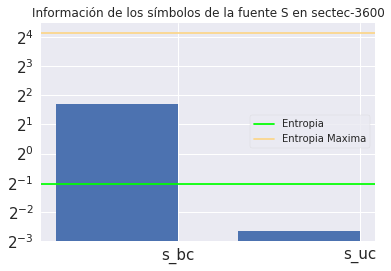
\includegraphics[page=1,width=.70\textwidth]{../img/sectec}
 \caption{Entropía de la red}
 \label{fig:barras-sectec}
\end{figure}


 \subsubsection{Grafo de conectividad de la red}


\begin{figure}[H]
   \centering
       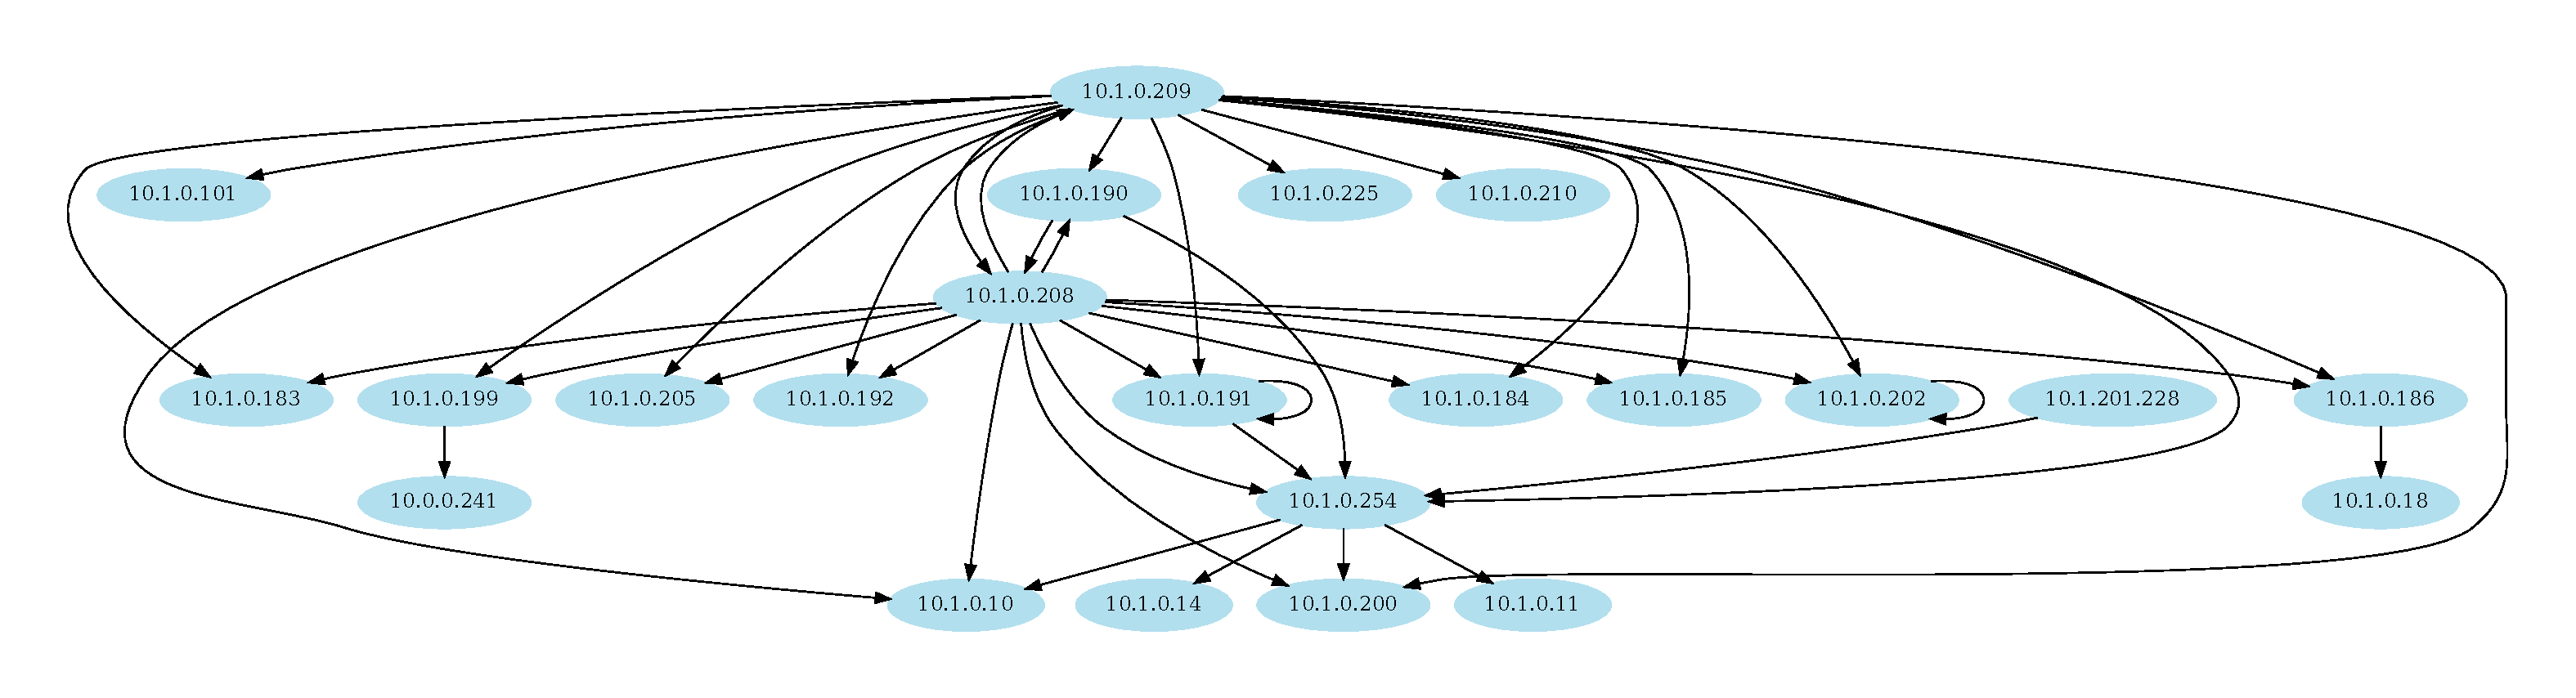
\includegraphics[page=1,height=8cm ,width=1.08\textwidth]{../img/red-sectec}
 \caption{Grafo de conectividad}
 \label{fig:grafo-sectec}
\end{figure}


\subsubsection{Información y nodos distinguidos}


Para esta sección reutilizamos la herramienta presentada en el ejercicio 2 con el objetivo de analizar la presencia de nodos distinguidos de la fuente. \\

\begin{figure}[H]
    \centering
    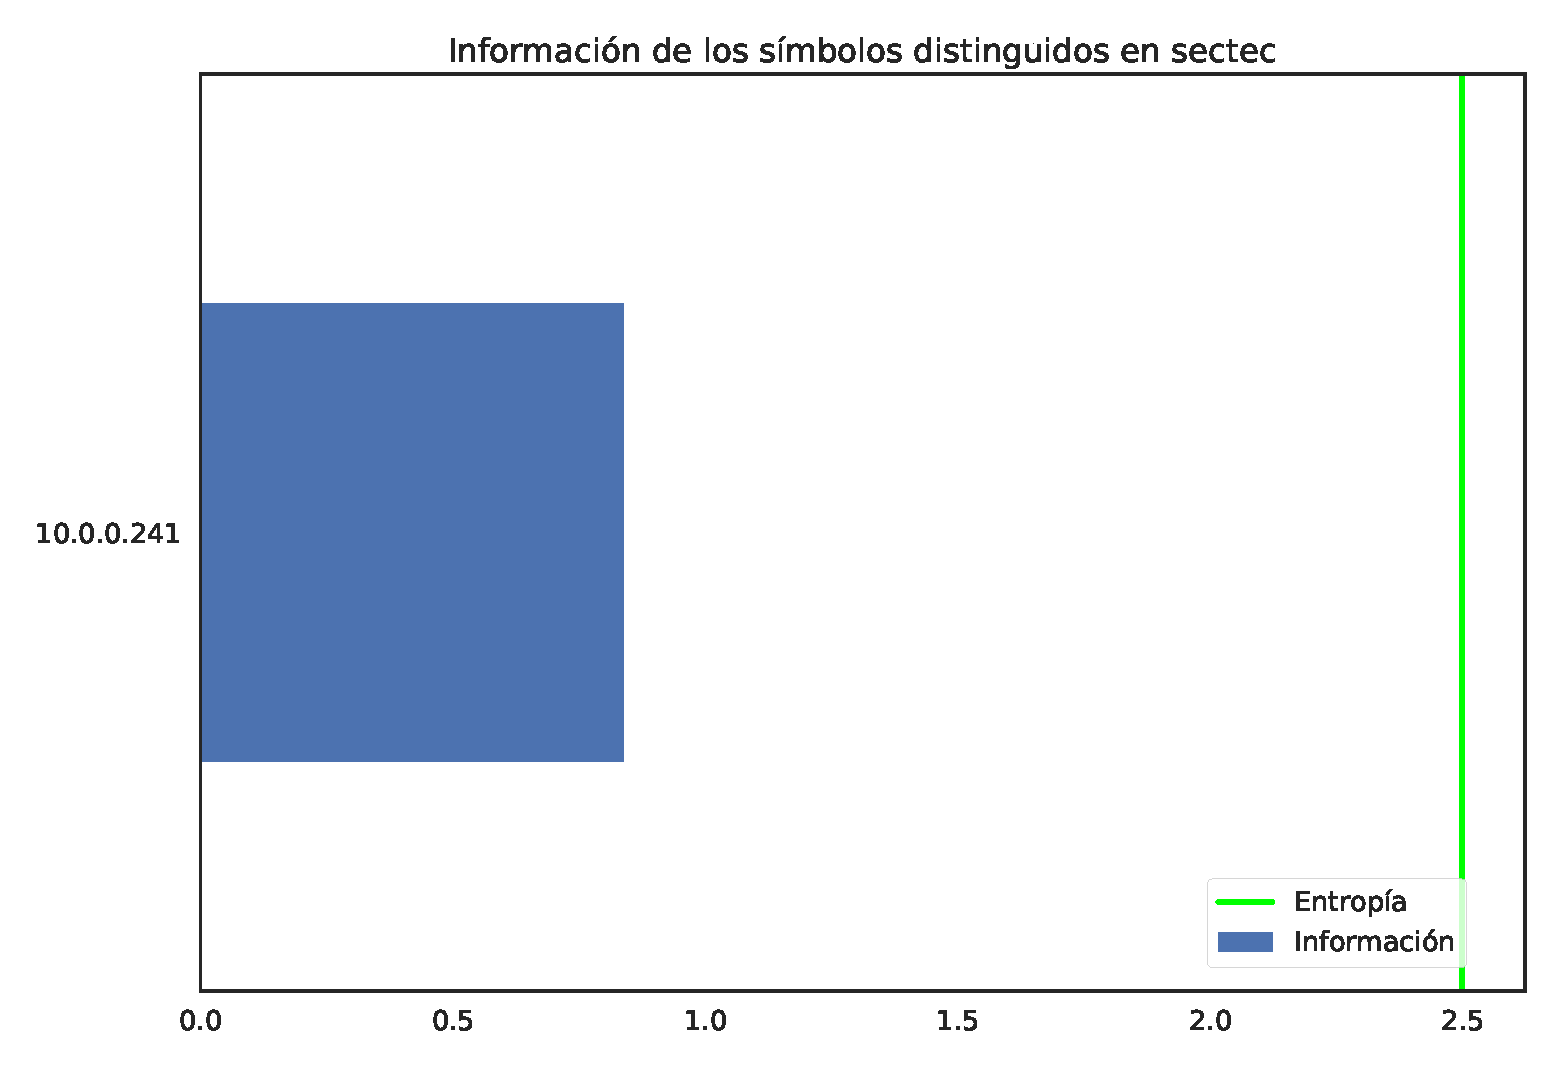
\includegraphics[page=1, height=6.55cm ,width=\textwidth]{../img/distinguidos-sectec}
    \caption{Nodos distinguidos}
    \label{fig:distinguidos-sectec}
\end{figure}
